Here we will try in an out-of-sample setting our preferred methods to see how they perform. We will only test the Average-drawdown based method and the Threshold-optimization one. The reasons for testing only those two models are various: first of all the Average-drawdown method is just an improvement of the simple sharpe-ranking method, achieving better results, so it doesn't make sense to test the less evoluted algorithm as well. The regression model will not be used as the performance was not enough good to the requirements we had and moreover it didn't allow us to control the output well enough. We therefore decided to stick with those models that seemed to be the best ones and try a full-out-of-sample test. This test will be run on the larger dataset (the one with 18000 trading pairs) from 2012 to the end of 2017. I will provide statistics for both the old in-sample window (2012-2015) and the new out-of-sample window (2016-2017).\\
Let's start from the average drawdown method. This one was optimized in-sample achieving a global performance in the area of 4.0 in terms of Sharpe-Ratio. The optimal parameters showed that the window to filter strategies should ideally be around 350 days, while the window to rank strategies based on their drawdown time should be a bit smaller. Let's see how it behaves in the out-of-sample period.\\
This is shown in the statistics for the total period showed in table \ref{table:tot_perf_av_drawdown} and the results for the out-of-sample period only in table \ref{table:oos_perf_av_drawdown}. The equity line can be found in \ref{Average_Drawdown_OOS}

\begin{table}
	\centering
	\begin{tabular}{c|c}
		\textbf{Statistic} & \textbf{Value} \\\hline
		Sharpe Ratio & 3.4269 \\ 
		Sortino Ratio & 3.8354 \\ 
		Omega Ratio & 2 \\ 
		Skewness & -0.6882 \\ 
		Kurtosis & 16.64 \\ 
		Maximum Drawdown (\% duration/duration) & 18 \\ 
		Longest Drawdown (days) & 197 \\ 
		Winning Days & 64.657 \\ 
	\end{tabular}
	\caption{\label{table:tot_perf_av_drawdown} Statistics for the total performance of the Average-Drawdown method.}
\end{table}


\begin{table}
	\centering
	\begin{tabular}{c|c}
		\textbf{Statistic} & \textbf{Value} \\\hline
		Sharpe Ratio & 0.8461 \\ 
		Sortino Ratio & 0.8206 \\ 
		Omega Ratio & 1.2 \\ 
		Skewness & -2.0903 \\ 
		Kurtosis & 26.18 \\ 
		Maximum Drawdown (\% duration/duration) & 37.8 \\ 
		Longest Drawdown (days) & 197 \\ 
		Winning Days & 58.92 \\ 
	\end{tabular}
	\label{table:oos_perf_av_drawdown}
	\caption{\label{table:oos_perf_av_drawdown} Performance Statistics for the out-of-sample period only of the Average-Drawdown method.}
\end{table}

\begin{center}
	\centering
	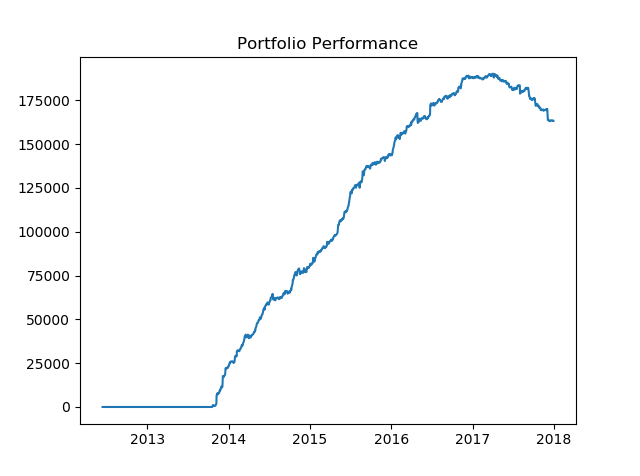
\includegraphics[width=0.6\textwidth]{GridSearches/Average_Drawdown/OOs_PnL_Line.png}
	\captionof{figure}{Out-of-sample Equity Line for the average-drawdown method}
	\label{Average_Drawdown_OOS}
\end{center}

We can see how there is a collapse of the performance. The overall statistics are quite good, but these are definitely lower than the in-sample ones. In the in-sample period the optimization worked really well, and the performance on the out-of-sample dataset in the 2012-2015 period is actually better than on the in-sample dataset thanks to the higher abundance of strategies. This is because when the strategies are more, it is easier to pick 50 good strategies by ranking them. It is interesting to notice how after mid-2016 the market radically changes (due to the effects of Brexit and the presidential elections in the United States) and many strategies stop working. This makes our optimization anachronistic and our models don't work any longer. This makes our drawdown-based method completely unapplicable in reality.\\
We hope that the threshold-optimization method will be able to survive the change in the market dynamics that occurred in 2016. We test it in the same fashion and the results are respectively shown in the following figures and tables \ref{table:tot_perf_threshold_backtest} and \ref{table:oos_perf_threshold_backtest}.

\begin{center}
	\centering
	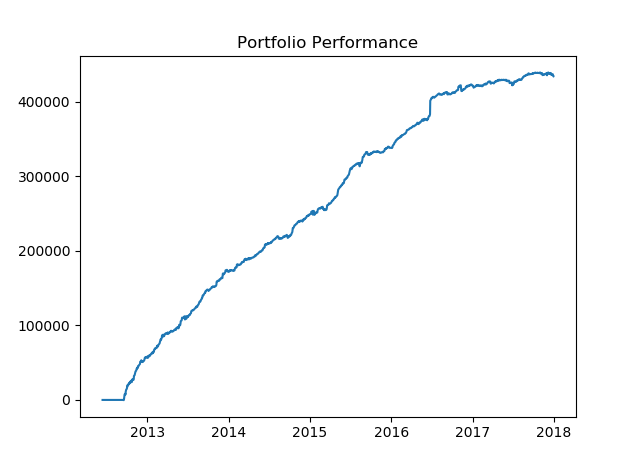
\includegraphics[width=0.6\textwidth]{GridSearches/Threshold_Backtest/PnL_Out_of_Sample.png}
	\captionof{figure}{\label{Threshold_Backtest_OOS} Out-of-sample Equity Line for the Threshold-Optimization method}
	
\end{center}

\begin{center}
	\centering
	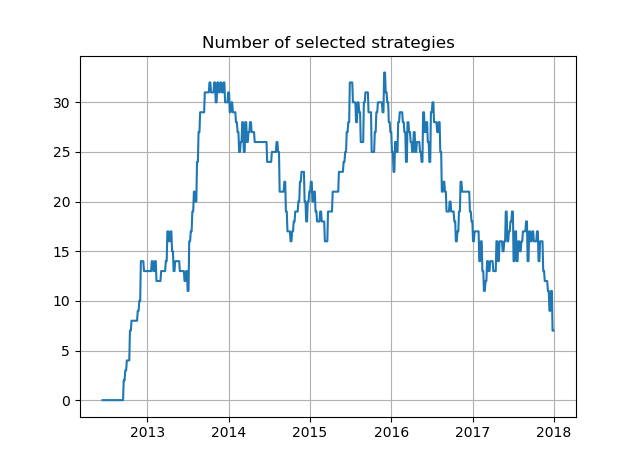
\includegraphics[width=0.6\textwidth]{GridSearches/Threshold_Backtest/num_strats_Out_of_Sample.png}
	\captionof{figure}{Out-of-sample number of strategies selected for the  Threshold-Optimization method}
	\label{Threshold_Backtest_OOS_n_strats}
\end{center}

\begin{table}
	\centering
	\begin{tabular}{c|c}
		\textbf{Statistic} & \textbf{Value} \\\hline
		Sharpe Ratio & 5.2342 \\ 
		Sortino Ratio & 7.6265 \\ 
		Omega Ratio & 3.06 \\ 
		Skewness & 4.6604 \\ 
		Kurtosis & 89.54 \\ 
		Maximum Drawdown (\% duration/duration) & 3.5 \\ 
		Longest Drawdown (days) & 48 \\ 
		Winning Days & 70.942 \\ 
	\end{tabular}
	\label{table:tot_perf_threshold_backtest}
	\caption{\label{table:tot_perf_threshold_backtest} Performance Statistics for the total period of the Threshold-Optimization method.}
\end{table}

\begin{table}
	\centering
	\begin{tabular}{c|c}
		\textbf{Statistic} & \textbf{Value} \\\hline
		Sharpe Ratio & 2.8255 \\ 
		Sortino Ratio & 5.068 \\ 
		Omega Ratio & 2.09 \\ 
		Skewness & 9.717 \\ 
		Kurtosis & 17.355 \\ 
		Maximum Drawdown (\% duration/duration) & 9.2 \\ 
		Longest Drawdown (days) & 48 \\ 
		Winning Days & 67.17 \\ 
	\end{tabular}
	\label{table:oos_perf_threshold_backtest}
	\caption{\label{table:oos_perf_threshold_backtest} Performance Statistics for the out-of-sample period only of the Threshold-Optimization method.}
\end{table}

We can see that there is still a drop in the performance in the second part of the out-of-sample period (the Sharpe drops from roughly 5 to 2.8). Anyway the model is still able to adapt and bring PnL even after this market change. Overall we consider this a very good result considering how challenging our task is, and we decide to stick with this method for further analysis. We can also see how the performance suffers in the end as the number of strategies selected drops significantly. This led us to reflect on the average behaviour of the strategies. It might in fact make sense that the performance of simple mean-reversion strategies decreases as time passes by as markets become more efficient and more players trade the same pairs as we do. Just to give a numerical taste to this feeling we plot the number of strategies that have a significant Sharpe-Ratio (more than 2) over a one-year window. 

\begin{center}
	\centering
	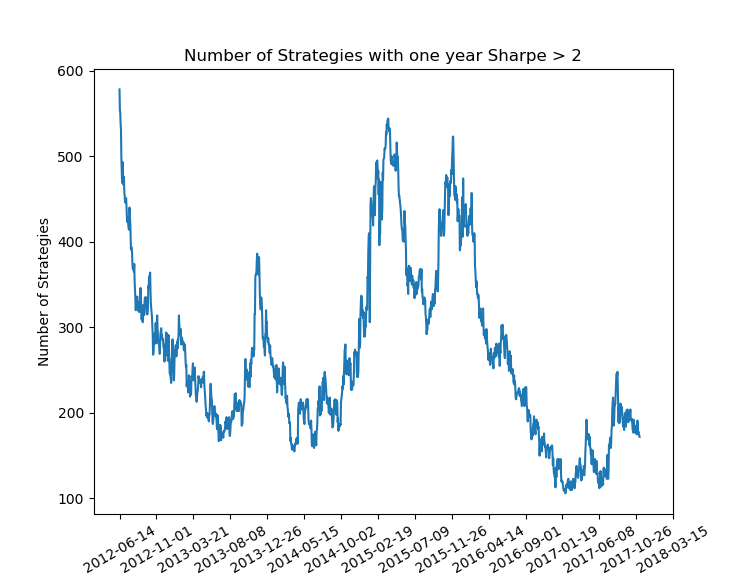
\includegraphics[width=0.6\textwidth]{Part_1/Number_of_Sharpes.png}
	\captionof{figure}{\label{Number_sharpes} Number of strategies that have a one-year Sharpe-Ratio above 2}
\end{center}

We can see as expected that the number of "good" strategies available drops significantly starting from the end of 2015. This confirms substantially the theory of decaying performance. Moreover this chart confirms how the market has changed from 2016 onwards. Of course, the methods struggle in such periods, moreover we can see how the good performance that many methods exhibit along 2014 can be explained by the abundance of well-performing strategies.


